\chapter{SIMD优化}
前面介绍的Athread是专为神威系统设计的原生并行计算库,属于神威系统中支持最好、功能最齐全的并行库。但是除Athread之外,神威系统中还有几个按照国际标准设计的标准并行计算库,比如OpenACC和MPI等,这些库存在的意义主要是适应各种不同的编程和优化需求,并且方便神威系统移植一些用标准库编写的软件,从而扩大神威系统的适用范围。SIMD就是这些库之一,比起Athread,SIMD技术发挥作用的系统层次更加偏向底层,其功能也更加简单。本章将着重于介绍神威系统中的SIMD技术,主要内容对应于《编译手册》第八章和《优化手册》5.4节。

\section{SIMD介绍}
\subsection{SIMD是什么}
SIMD全称单指令流多数据流(SingleInstruction Multiple Data),是一种同时对一组数据(又称“数据向量”)分别执行相同的操作的并行技术,即利用数据级并行来提高计算效率。SIMD和上一章所讲的多线程从核并行类似\footnote{回忆一下athread\_spawn()函数},都是让大量相同的操作在同一时间段内并发进行。但SIMD与多线程从核并行的区别主要来自以下两点:
\begin{itemize}
	\item SIMD将要并行处理的数据存放于\textbf{寄存器}中,从核并行将数据读入到从核内存;
	\item SIMD的并行是\textbf{指令}的并行(即每执行一条指令时都同时复制给多个数据执行),多线程从核并行是线程(把多个指令组成的一段程序整个复制到多个从核上执行)的并行。
\end{itemize}

可以看出SIMD虽然和前面介绍的从核并行有很多相似点,但是其实它们的实现是完全不同的。SIMD目前使用广泛的领域主要是多媒体文件处理。Intel家的SIMD技术有MMX和SSE\footnote{这些技术起初是用SIMD加速多媒体文件的处理过程,现在经常可以在一些深度学习框架的编译选项中发现这些东西};AMD家的有3D Now!技术\footnote{也是个多媒体指令集。顾名思义,和三维图像处理有关的}等。

\subsection{神威系统中的SIMD介绍}
\subsubsection{支持的运算}
申威26010处理器的主核和从核都支持SIMD,且支持的SIMD宽度都是256位,支持的操作如表\ref{tab:神威系统SIMD支持的运算}。
\begin{table}[!htbp]
	\caption{神威系统SIMD支持的运算}\label{tab:神威系统SIMD支持的运算}
	\centering
	\footnotesize% fontsize
	\setlength{\tabcolsep}{4pt}% column separation
	\renewcommand{\arraystretch}{1.2}%row space 
	\begin{tabular}{|c|c|c|c|c|}
		\hline
		\diagbox{运算类型}{支持运算} & 逻辑    & 移位    & 加减     & 乘除     \\
		\hline
		8个32位定点运算              & $\surd$ & $\surd$ & $\surd$  & $\times$ \\
		\hline
		1个256位定点运算             & $\surd$ & $\surd$ & $\times$ & $\times$ \\
		\hline
		4个64位定点运算              & $\surd$ & $\surd$ & $\surd$  & $\surd$  \\
		\hline
	\end{tabular}
\end{table}

\subsubsection{使用形式}
神威编译器在C语言上扩展了一些SIMD数据类型和函数,扩展的函数基本都是直接映射到SIMD指令,在编译时由编译器自动进行inline,因此编程时不需要了解具体的SIMD指令,只需要调用函数即可进行SIMD操作。神威编译器的C语言SIMD扩展可以在C语言一级获得与汇编程序一样的性能。

\section{神威SIMD使用入门}
\subsection{SIMD数据类型}
神威编译器SIMD扩展的数据类型如表\ref{tab:神威编译器SIMD扩展数据类型}。注意SIMD扩展数据类型本质只是多个基本数据类型的拼接,但是和C语言中的\code{int}、\code{int}等类型一样是值类型而不是像\code{int[8]}、\code{float[4]}一样的指针类型。
\begin{table}[!htbp]
	\caption{神威编译器SIMD扩展数据类型}\label{tab:神威编译器SIMD扩展数据类型}
	\centering
	\footnotesize% fontsize
	\setlength{\tabcolsep}{4pt}% column separation
	\renewcommand{\arraystretch}{1.2}%row space 
	\begin{tabular}{|c|c|}
		\hline
		类型            & 含义                 \\
		\hline
		\code{intv8}    & 8个32位有符号整型    \\
		\hline
		\code{uintv8}   & 8个32位无符号整型    \\
		\hline
		\code{int256}   & 1个256位有符号长整型 \\
		\hline
		\code{uint256}  & 1个256位无符号长整型 \\
		\hline
		\code{floatv4}  & 4个64位单精度浮点    \\
		\hline
		\code{doublev4} & 4个64位双精度浮点    \\
		\hline
	\end{tabular}
\end{table}

\subsection{SIMD的等号赋值和数据转换}
\subsubsection{标准类型到SIMD扩展类型等号赋值}
标准类型到SIMD扩展类型的赋值是以值扩展方式进行的,具体规则如下:
\begin{itemize}
	\item 标准类型到\code{int256}型:先转化为\code{long}型然后把值复制到低64位,符号位复制到高192位;
	\item 标准类型到非\code{int256}型:先转化为扩展类型对应的标准类型再\textbf{复制}指定份数放入扩展类型中。例如变量\code{floatv4 fv; int iv;}的赋值\code{fv=iv;}或\code{fv=1;}是先将\code{iv}或整型常数1转化为浮点型再复制4份放入\code{fv}中;
	\item 数组赋值:例如数据类型\code{floatv4 fv;}可以有\code{fv = \{1.0,2,3.0\};}这样的赋值,数组赋值从低位到高位,缺省补0,其赋值结果为:
	      \begin{center}
		      \begin{tabular}{|c|c|c|c|}
			      \hline
			      192$\sim$255位 & 128$\sim$191位 & 64$\sim$127位 & 0$\sim$63位 \\
			      \hline
			      0              & 3.0            & 2.0           & 1.0         \\
			      \hline
		      \end{tabular}
	      \end{center}
	      又比如数组\code{float fs[4]}可以有\code{floatv4* fv = (floatv4*)(\&fs[0]);}\footnote{这条语句如何理解?指针很有趣,请结合前文所讲的扩展类型的本质仔细揣摩。有疑问请看《编译手册》8.3.6节}。
\end{itemize}

\subsubsection{SIMD扩展类型之间等号赋值}
SIMD数据互相之间赋值是以传值模式进行的。相同数据类型的SIMD数据互相赋值和正常的C语言赋值一样,不同类型的数据赋值语句的数据转换规则如下所示:
\begin{itemize}
	\item floatv4和doublev4赋值:单精度和双精度浮点数扩展类型互相赋值时会自动进行数据类型的转换,源扩展类型值中的每个数分别转换后放入目的扩展类型中;
	\item int256和intv8/uintv8:256位整型和8个32位整型互相赋值时没有数据类型的转换,数据不发生任何变化。
\end{itemize}

\subsubsection{SIMD扩展类型到标准类型等号赋值}
只取扩展类型最低位的部分。

\subsection{SIMD宏赋值}
宏赋值就比较好理解了,就是向一个宏定义中“输入”几个数得到存入这些数的扩展类型。

\subsubsection{输入多个数的赋值宏}
这类宏接受几个独立的数值,返回存入这些数的扩展类型,具体的宏如表\ref{tab:神威编译器中输入多个数的SIMD赋值宏}。
\begin{table}[!htbp]
	\caption{神威编译器中输入多个数的SIMD赋值宏}\label{tab:神威编译器中输入多个数的SIMD赋值宏}
	\centering
	\footnotesize% fontsize
	\setlength{\tabcolsep}{4pt}% column separation
	\renewcommand{\arraystretch}{1.2}%row space 
	\begin{tabular}{|c|c|c|}
		\hline
		宏定义                          & 输入参数                & 输出类型        \\
		\hline
		\code{simd\_set\_intv8(...)}    & 8个\code{int}           & \code{intv8}    \\
		\hline
		\code{simd\_set\_uintv8(...)}   & 8个\code{unsigned int}  & \code{uintv8}   \\
		\hline
		\code{simd\_set\_int256(...)}   & 4个\code{long}          & \code{int256}   \\
		\hline
		\code{simd\_set\_uint256(...)}  & 4个\code{unsigned long} & \code{uint256}  \\
		\hline
		\code{simd\_set\_floatv4(...)}  & 4个\code{float}         & \code{floatv4}  \\
		\hline
		\code{simd\_set\_doublev4(...)} & 4个\code{double}        & \code{doublev4} \\
		\hline
	\end{tabular}
\end{table}

\subsubsection{输入数组首地址的赋值宏}
比起用上面介绍的输入多个数的赋值宏,在并行优化中一般更倾向于使用速度更快\footnote{显而易见,输入单个数赋值需要对内存空间的离散访问,而输入数组的意味着访问连续存储,速度势必会更快}的输入数组首地址的赋值宏对扩展数据类型进行赋值。具体的宏如表\ref{tab:神威编译器中输入数组首地址的SIMD赋值宏}。其中\code{simd\_load(.,.)}和\code{simd\_store(.,.)}要求\textbf{对界},即输入的数组起始位置必须是数组起点的第$256\times n(n\in\mathbf{N})$位\footnote{不对界的访问会引起异常,然后由操作系统模拟,产生很大的性能损失};而\code{simd\_loadu(.,.)}和\code{simd\_storeu(.,.)}不要求对界存储。这两个赋值宏一般搭配使用。

输入数组首地址的赋值宏一次必须读取256位。在实际的优化中,如果要输入的数组在计算到最后末尾不足256位,一般来说直接将剩下的数据直接串行计算或从末尾开始读最后的数据即可。

\begin{table}[!htbp]
	\caption{神威编译器中输入数组首地址的SIMD赋值宏}\label{tab:神威编译器中输入数组首地址的SIMD赋值宏}
	\centering
	\footnotesize% fontsize
	\setlength{\tabcolsep}{4pt}% column separation
	\renewcommand{\arraystretch}{1.2}%row space 
	\begin{tabular}{|c|p{8cm}<{\centering}|p{2.5cm}<{\centering}|}
		\hline
		宏定义                  & 对应操作                                                                                                                                   & 输入参数 \\
		\hline
		\tabincell{c}{\code{simd\_load(.,.)}                                                                                                                                           \\ \code{simd\_loadu(.,.)}}  & 从输入的数组首地址开始读取256位数据装入输入的扩展类型变量中                                                                                & \multirow{3}{3cm}{扩展类型变量\footnote{注意这里不是填地址},\\数组首地址\footnote{即\code{\&数组名[起始位置]}形式}} \\
		\cline{1-2}
		\code{simd\_loade(.,.)} & 如果输入的扩展类型变量是浮点型,则从输入的数组首地址开始读取64位数据复制4份装入输入的扩展类型变量中,否则若是整型则读取32位数据复制8份装入 &          \\
		\cline{1-2}
		\tabincell{c}{\code{simd\_store(.,.)}                                                                                                                                            \\ \code{simd\_storeu(.,.)}} & 将扩展类型变量中的值写入到从输入的数组首地址开始的256位中                                                                                  &                                                                                                \\
		\hline
	\end{tabular}
\end{table}

\subsection{SIMD数据输出宏}
\begin{itemize}
	\item 控制台输出,效果同\code{printf("[ \%d, \%d, \%d, \%d, \%d, \%d, \%d, \%d ]", v[7], v[6], v[5], v[4], v[3], v[2], v[1], v[0])}或\code{printf("[ \%f, \%f, \%f, \%f ]", v[3], v[2], v[1], v[0])},不同的函数对应以不同的数据类型输出。输出字符串为以方括号包围的多个数,数字之间以逗号分隔;
	\item 文件输出,效果同\code{fprintf(file, "[ \%d, \%d, \%d, \%d, \%d, \%d, \%d, \%d ]", v[7], v[6], v[5], v[4], v[3], v[2], v[1], v[0])}或\code{fprintf(file, "[ \%f, \%f, \%f, \%f ]", v[3], v[2], v[1], v[0])},输出字符串格式同上。
\end{itemize}

其宏定义如表\ref{tab:神威编译器SIMD输出操作宏定义}所示。
\begin{table}[!htbp]
	\caption{神威编译器SIMD输出操作宏定义}\label{tab:神威编译器SIMD输出操作宏定义}
	\centering
	\footnotesize% fontsize
	\setlength{\tabcolsep}{4pt}% column separation
	\renewcommand{\arraystretch}{1.2}%row space 
	\begin{tabular}{|c|c|c|}
		\hline
		控制台输出宏                      & 文件输出宏                               & 对应的类型      \\
		\hline
		\code{simd\_print\_intv8(...)}    & \code{simd\_fprint\_intv8(FILE*,...)}    & \code{intv8}    \\
		\hline
		\code{simd\_print\_uintv8(...)}   & \code{simd\_fprint\_uintv8(FILE*,...)}   & \code{uintv8}   \\
		\hline
		\code{simd\_print\_int256(...)}   & \code{simd\_fprint\_int256(FILE*,...)}   & \code{int256}   \\
		\hline
		\code{simd\_print\_uint256(...)}  & \code{simd\_fprint\_uint256(FILE*,...)}  & \code{uint256}  \\
		\hline
		\code{simd\_print\_floatv4(...)}  & \code{simd\_fprint\_floatv4(FILE*,...)}  & \code{floatv4}  \\
		\hline
		\code{simd\_print\_doublev4(...)} & \code{simd\_fprint\_doublev4(FILE*,...)} & \code{doublev4} \\
		\hline
	\end{tabular}
\end{table}

\subsection{SIMD运算}
SIMD运算有运算符和运算宏两种实现方式,这两种实现方式是等价的,但是运算符只能执行一部分运算,运算宏能执行所有支持的运算。基本的算术运算、逻辑运算、位运算的运算符和宏如表\ref{tab:神威编译器SIMD基本运算符宏定义}。支持的全部运算宏定义请见《编译手册》8.5.3和8.5.4节。

\begin{table}[!htbp]
	\caption{神威编译器SIMD基本算术运算符宏定义}\label{tab:神威编译器SIMD基本运算符宏定义}
	\centering
	\footnotesize% fontsize
	\setlength{\tabcolsep}{4pt}% column separation
	\renewcommand{\arraystretch}{1.2}%row space 
	\begin{tabular}{|c|c|c|c|c|}
		\hline
		运算   & \diagbox{符}{宏}{类型} & \code{intv8}       & \code{floatv4}     & \code{doublev4}    \\
		\hline
		加     & +                      & \code{simd\_vaddw} & \code{simd\_vadds} & \code{simd\_vaddd} \\
		\hline
		减     & -                      & \code{simd\_vsubw} & \code{simd\_vsubs} & \code{simd\_vsubd} \\
		\hline
		乘     & *                      & 无                 & \code{simd\_vmuls} & \code{simd\_vmuld} \\
		\hline
		除     & 无                     & 无                 & \code{simd\_vdivs} & \code{simd\_vdivd} \\
		\hline
		按位与 & \&                     & \code{simd\_vandw} & 无                 & 无                 \\
		\hline
		按位或 & |                      & \code{simd\_vbisw} & 无                 & 无                 \\
		\hline
		异或   & \^{}                   & \code{simd\_vxorw} & 无                 & 无                 \\
		\hline
		左移   & <<                     & \code{simd\_vsllw} & 无                 & 无                 \\
		\hline
		右移   & >>                     & \code{simd\_vsrlw} & 无                 & 无                 \\
		\hline
	\end{tabular}
\end{table}

\section{神威SIMD优化示例}
SIMD基础学会了就可以拿来进行实际的优化了。本节将使用SIMD对\ref{subsec:并行编程思路}节的参考程序(附录\ref{apdx:第一个程序})进行进一步的优化。

\ref{subsec:并行编程思路}节的程序中,只有从核在进行并行计算,因此SIMD优化只需要在从核代码上进行。其基本思路如下:
\begin{enumerate}
	\item 循环分裂:将从核代码中的循环分裂为子循环,每个子循环由8个\code{int}加法组成;
	\item 变量提取:将子循环中的8个加法操作的加数变量和结果变量提取出来,用simd\_load分别装载到SIMD扩展变量中;
	\item 计算:执行SIMD加法运算;
	\item 结果写回:用simd\_store将计算结果从SIMD扩展变量写回结果数组中。
\end{enumerate}

以此编写的程序如附录\ref{apdx:优化后的第一个程序从核}所示。此外,神威编译器编译带有SIMD库的程序时需要加上\code{-msimd}编译选项,将该选项加在Makefile(见\ref{subsec:编写Makefile}节)从核编译指令后即可。

依然是命令行打\code{make run}运行程序,如果一切正常,可以看到SIMD优化后的程序和\ref{subsec:并行编程思路}节原本的并行程序相比性能提升并不明显,这是由于在矩阵相加运算中,并行程序的主要时间消耗在\code{athread\_get}和\code{athread\_put}读写数据的DMA操作上,而SIMD是对计算过程的优化,因此优化效果不明显。

\section{本章总结}
\subsection{知识点概括}
本章主要讲解的神威系统中SIMD的使用,主要知识点如图\ref{fig:Chap_SIMD}所示。

\begin{figure}[!htbp]
	\centering
	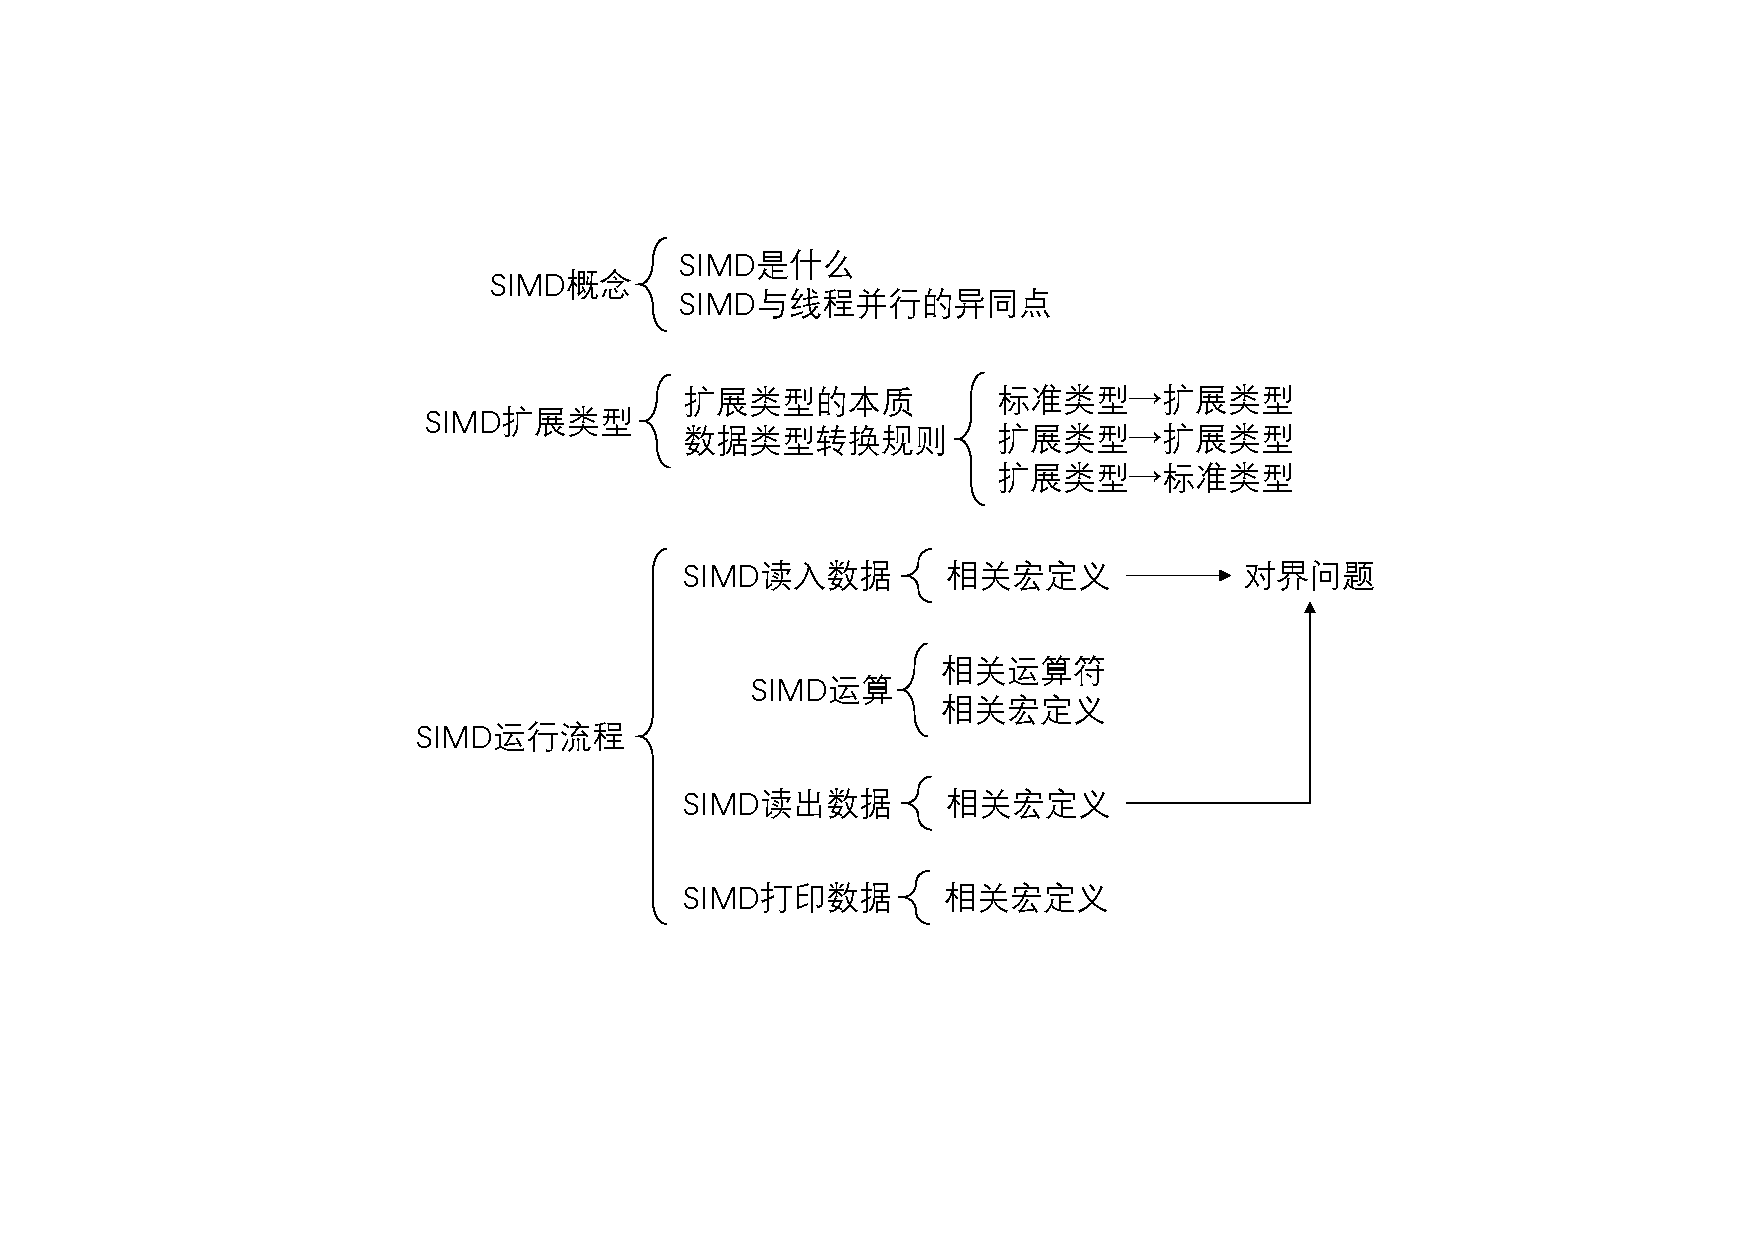
\includegraphics[width=\textwidth]{Chap_SIMD}
	\caption{第\thechapter{}章的知识点概括}
	\label{fig:Chap_SIMD}
\end{figure}

\subsection{练习}
\begin{itemize}
	\item 用Athread实现并行的矩阵减法,并用SIMD优化之;
	\item 用Athread实现并行的矩阵乘法,并用SIMD优化之。
\end{itemize}